\documentclass[journal, a4paper]{IEEEtran}

% some very useful LaTeX packages include:

%\usepackage{cite}      % Written by Donald Arseneau
                        % V1.6 and later of IEEEtran pre-defines the format
                        % of the cite.sty package \cite{} output to follow
                        % that of IEEE. Loading the cite package will
                        % result in citation numbers being automatically
                        % sorted and properly "ranged". i.e.,
                        % [1], [9], [2], [7], [5], [6]
                        % (without using cite.sty)
                        % will become:
                        % [1], [2], [5]--[7], [9] (using cite.sty)
                        % cite.sty's \cite will automatically add leading
                        % space, if needed. Use cite.sty's noadjust option
                        % (cite.sty V3.8 and later) if you want to turn this
                        % off. cite.sty is already installed on most LaTeX
                        % systems. The latest version can be obtained at:
                        % http://www.ctan.org/tex-archive/macros/latex/contrib/supported/cite/

\usepackage{graphicx}   % Written by David Carlisle and Sebastian Rahtz
                        % Required if you want graphics, photos, etc.
                        % graphicx.sty is already installed on most LaTeX
                        % systems. The latest version and documentation can
                        % be obtained at:
                        % http://www.ctan.org/tex-archive/macros/latex/required/graphics/
                        % Another good source of documentation is "Using
                        % Imported Graphics in LaTeX2e" by Keith Reckdahl
                        % which can be found as esplatex.ps and epslatex.pdf
                        % at: http://www.ctan.org/tex-archive/info/

%\usepackage{psfrag}    % Written by Craig Barratt, Michael C. Grant,
                        % and David Carlisle
                        % This package allows you to substitute LaTeX
                        % commands for text in imported EPS graphic files.
                        % In this way, LaTeX symbols can be placed into
                        % graphics that have been generated by other
                        % applications. You must use latex->dvips->ps2pdf
                        % workflow (not direct pdf output from pdflatex) if
                        % you wish to use this capability because it works
                        % via some PostScript tricks. Alternatively, the
                        % graphics could be processed as separate files via
                        % psfrag and dvips, then converted to PDF for
                        % inclusion in the main file which uses pdflatex.
                        % Docs are in "The PSfrag System" by Michael C. Grant
                        % and David Carlisle. There is also some information
                        % about using psfrag in "Using Imported Graphics in
                        % LaTeX2e" by Keith Reckdahl which documents the
                        % graphicx package (see above). The psfrag package
                        % and documentation can be obtained at:
                        % http://www.ctan.org/tex-archive/macros/latex/contrib/supported/psfrag/

%\usepackage{subfigure} % Written by Steven Douglas Cochran
                        % This package makes it easy to put subfigures
                        % in your figures. i.e., "figure 1a and 1b"
                        % Docs are in "Using Imported Graphics in LaTeX2e"
                        % by Keith Reckdahl which also documents the graphicx
                        % package (see above). subfigure.sty is already
                        % installed on most LaTeX systems. The latest version
                        % and documentation can be obtained at:
                        % http://www.ctan.org/tex-archive/macros/latex/contrib/supported/subfigure/

\usepackage{url}        % Written by Donald Arseneau
                        % Provides better support for handling and breaking
                        % URLs. url.sty is already installed on most LaTeX
                        % systems. The latest version can be obtained at:
                        % http://www.ctan.org/tex-archive/macros/latex/contrib/other/misc/
                        % Read the url.sty source comments for usage information.

%\usepackage{stfloats}  % Written by Sigitas Tolusis
                        % Gives LaTeX2e the ability to do double column
                        % floats at the bottom of the page as well as the top.
                        % (e.g., "\begin{figure*}[!b]" is not normally
                        % possible in LaTeX2e). This is an invasive package
                        % which rewrites many portions of the LaTeX2e output
                        % routines. It may not work with other packages that
                        % modify the LaTeX2e output routine and/or with other
                        % versions of LaTeX. The latest version and
                        % documentation can be obtained at:
                        % http://www.ctan.org/tex-archive/macros/latex/contrib/supported/sttools/
                        % Documentation is contained in the stfloats.sty
                        % comments as well as in the presfull.pdf file.
                        % Do not use the stfloats baselinefloat ability as
                        % IEEE does not allow \baselineskip to stretch.
                        % Authors submitting work to the IEEE should note
                        % that IEEE rarely uses double column equations and
                        % that authors should try to avoid such use.
                        % Do not be tempted to use the cuted.sty or
                        % midfloat.sty package (by the same author) as IEEE
                        % does not format its papers in such ways.

\usepackage{amsmath}    % From the American Mathematical Society
                        % A popular package that provides many helpful commands
                        % for dealing with mathematics. Note that the AMSmath
                        % package sets \interdisplaylinepenalty to 10000 thus
                        % preventing page breaks from occurring within multiline
                        % equations. Use:
%\interdisplaylinepenalty=2500
                        % after loading amsmath to restore such page breaks
                        % as IEEEtran.cls normally does. amsmath.sty is already
                        % installed on most LaTeX systems. The latest version
                        % and documentation can be obtained at:
                        % http://www.ctan.org/tex-archive/macros/latex/required/amslatex/math/
\usepackage{listings}
\usepackage{color}

\definecolor{dkgreen}{rgb}{0,0.6,0}
\definecolor{gray}{rgb}{0.5,0.5,0.5}
\definecolor{mauve}{rgb}{0.58,0,0.82}

\lstset{frame=tb,
  language=Java,
  aboveskip=3mm,
  belowskip=3mm,
  showstringspaces=false,
  columns=flexible,
  basicstyle={\small\ttfamily},
  numbers=none,
  numberstyle=\tiny\color{gray},
%   keywordstyle=\color{blue},
%   commentstyle=\color{dkgreen},
%   stringstyle=\color{mauve},
  breaklines=true,
  breakatwhitespace=true,
  tabsize=3
}

% Other popular packages for formatting tables and equations include:

%\usepackage{array}
% Frank Mittelbach's and David Carlisle's array.sty which improves the
% LaTeX2e array and tabular environments to provide better appearances and
% additional user controls. array.sty is already installed on most systems.
% The latest version and documentation can be obtained at:
% http://www.ctan.org/tex-archive/macros/latex/required/tools/

% V1.6 of IEEEtran contains the IEEEeqnarray family of commands that can
% be used to generate multiline equations as well as matrices, tables, etc.

% Also of notable interest:
% Scott Pakin's eqparbox package for creating (automatically sized) equal
% width boxes. Available:
% http://www.ctan.org/tex-archive/macros/latex/contrib/supported/eqparbox/

% *** Do not adjust lengths that control margins, column widths, etc. ***
% *** Do not use packages that alter fonts (such as pslatex).         ***
% There should be no need to do such things with IEEEtran.cls V1.6 and later.


% Your document starts here!
\begin{document}
\begin{titlepage}

\newcommand{\HRule}{\rule{\linewidth}{0.5mm}} % Defines a new command for the horizontal lines, change thickness here

\center % Center everything on the page
 %----------------------------------------------------------------------------------------
%	LOGO SECTION
%----------------------------------------------------------------------------------------

~\\[1cm]

\includegraphics{SCUT.png}\\[2cm] % Include a department/university logo - this will require the graphicx package

%----------------------------------------------------------------------------------------
%	TITLE SECTION
%----------------------------------------------------------------------------------------

\HRule \\[1cm]
{ \huge \bfseries The Experiment Report of \textit{Machine Learning} }\\[0.6cm] % Title of your document
\HRule \\[2cm]
%----------------------------------------------------------------------------------------
%	HEADING SECTIONS
%----------------------------------------------------------------------------------------


\textsc{\LARGE \textbf{School:} School of Software Engineering}\\[1cm]
\textsc{\LARGE \textbf{Subject:} Software Engineering}\\[2cm] 

 
%----------------------------------------------------------------------------------------
%	AUTHOR SECTION
%----------------------------------------------------------------------------------------

\begin{minipage}{0.4\textwidth}
\begin{flushleft} \large
\emph{Author:}\\
Jining He % Your name
\end{flushleft}
\end{minipage}
~
\begin{minipage}{0.4\textwidth}
\begin{flushright} \large
\emph{Supervisor:} \\
Qingyao Wu % Supervisor's Name
\end{flushright}
\end{minipage}\\[2cm]
~
\begin{minipage}{0.4\textwidth}
\begin{flushleft} \large
\emph{Student ID:}\\
201721045565
\end{flushleft}
\end{minipage}
~
\begin{minipage}{0.4\textwidth}
\begin{flushright} \large
\emph{Grade:} \\
Graduate
\end{flushright}
\end{minipage}\\[2cm]

% If you don't want a supervisor, uncomment the two lines below and remove the section above
%\Large \emph{Author:}\\
%John \textsc{Smith}\\[3cm] % Your name

%----------------------------------------------------------------------------------------
%	DATE SECTION
%----------------------------------------------------------------------------------------

{\large \today}\\[2cm] % Date, change the \today to a set date if you want to be precise

 
%----------------------------------------------------------------------------------------

\vfill % Fill the rest of the page with whitespace

\end{titlepage}

% Define document title and author
	\title{Linear Regression, Linear Classification and Gradient Descent}
	\maketitle

% Write abstract here
\begin{abstract}
This report show that how to use gradient descent to optimize linear regression and linear classification on small dataset.
% The short abstract is intended to give the reader an overview of the experiment. It should be brief and to the point. 
\end{abstract}

% Each section begins with a \section{title} command
\section{Introduction}
	% \PARstart{}{} creates a tall first letter for this first paragraph
% \PARstart{T}{his} section introduces the problem to solved and leads the reader on to the main part. Detailed motivation is necessary. What's more, you can show your expected results and contributions.
\PARstart{T}{his} experiment let us solve two problems. 
The first one requires us to predict the price of house. 
The second one requires us to distinguish whether or not Australians.

The Motivation of this experiment is let us further understand of linear regression and gradient descent,conduct some experiments under small scale dataset and realize the process of optimization and adjusting parameters.

% 这个实验让我们练习线性回归、线性分类、梯度下降,目的是
% 进一步理解线性回归和梯度下降的原理。
% 在小规模数据集上实践。
% 体会优化和调参的过程。


% Main Part
\section{Methods and Theory}
% In this section, you are asked to give a complete introduction to the experiment. For instance, the chosen methods, the related theories, the related equations(loss function), the derivation process(taking the gradient) and so on.
In this experiment, we use linear regression to predict the price of house and use SVM as linear classifier to distinguish whether or not Australians.

In linear regression, the loss function we used is:
\begin{equation} \label{eq:linear regression loss function}
    J(W,b) = \frac{1}{2m}\sum_{i=1}^m(y_i-(W^Tx_i+b))^2
\end{equation} 
The gradient formulas are:
\begin{equation} \label{eq:linear regression gradient formula}
    \begin{aligned}
        fff \\
        ff
        % g_w &= X(W^TX+b-Y)\\
        % g_b &= \frac{1}m\sum_{i=1}^m(W^Tx_i-y_i)
    \end{aligned}
\end{equation}

In linear classification, we add hinge loss to our loss function:
\begin{equation} \label{eq:linear classification loss function}
    J(W,b) = \frac{||W||^2}2+\frac{C}m\sum_{i=1}^{m}max(0,1-y_i(W^Tx_i+b))
\end{equation}
The gradient formulas are:
\begin{equation} \label{eq:linear classification gradient formula}
    \begin{aligned}
        \nabla_WJ(W,b) &= W+\frac{C}m\sum_{i=1}^{m}g_W(x_i)\\
        \nabla_bJ(W,b) &= \frac{C}m\sum_{i=1}^{m}g_b(x_i)
    \end{aligned}
\end{equation}

We update both models using below:
\begin{equation} \label{eq:update parameters formula}
    \begin{aligned}
        W&=W-\alpha \nabla_WJ(W,b)\\
        b&=b-\alpha \nabla_bJ(W,b)
    \end{aligned}
\end{equation}


% 在本次实验中,我们使用线性回归来预测房屋价格,使用线性分类判断是否为澳大利亚人。
% 在线性回归中,我们使用的Loss Function为
% 梯度为

% 在线性分类中,我们使用SVM分类器,higo loss, LossFunction为
% 梯度为

% This experiment let us learn Linear Regression and Linear Classification. 

% Linear Regression
% loss function
% gradient formula

% Linear Classification
% loss function
% gradient formula


\section{Experiments}
\subsection{Dataset}
% 实验数据集来自,线性回归使用数据集,包含了,线性分类使用数据集,包含了
The datasets are from LIBSVM.
Linear Regression uses Housing dataset, including 506 samples and each sample has 13 features.
Linear classification uses australian dataset, including 690 samples and each sample has 14 features.
We use scaled edition directly.
% This section represents the related information of datasets, such as the content, the number of data, the training set, the validation set and so on.

\subsection{Implementation}
% All detailed implementation in your experiment: initialization, process, results, all kinds of parameters. In a word, describe clearly What you do and how you do.\par

\subsubsection{Data Preprocessing}
Use load\textunderscore svmlight\textunderscore file function in sklearn library to load the dataset.
Divide dataset into training set and validation set using train\textunderscore test\textunderscore split function.
The division ratio is 4 to 1.
I also convert data to column vector.

% 使用sklearn库中的load_svmlight_fileh函数加载数据集。
% 使用train_test_split函数将数据集划分为训练集和验证集,使用4:1的比例。
% 将所有的向量转化为列向量
% Use load_svmlight_file function in sklearn library to load the experiment data.
% Divide dataset into training set and validation set using train_test_split function.

\subsubsection{Initialization}
There are many ways to initialize linear model parameters.
I choose to set all parameter into zero.
% 有多种方法初始化参数,在这里,我们使用零初初始化参数W,b。
% Initialize linear model parameters. You can choose to set all parameter into zero, initialize it randomly or with normal distribution.
\subsubsection{Compute Loss and Gradient} \label{compute loss and gradient}
In linear regression, use formula \eqref{eq:linear regression loss function} to compute loss and formula \eqref{eq:linear regression gradient formula} to compute gradient.
In linear classification, use formula \eqref{eq:linear classification loss function} to compute loss and formula \eqref{eq:linear classification gradient formula} to compute gradient.

% 使用公式求loss function 
% 在Linear Regression 我们采用的Loss Function为
% 在LInear Classification 我们的lossfunction为
% Loss function
% \subsubsection{Gradient}
% 使用公式求梯度
% 在Linear Regression 梯度公式为
% 在LInear Classification 梯度公式为
% calulate gradient 





\subsubsection{Update Parameters} \label{update parameters}
Use formula \eqref{eq:update parameters formula} to update parameters.
% Update parameters using 
% 更新参数公式
% update parameters using $$ W = W - \alpha G_W $$ $$ b = b - \alpha G_b $$
\subsubsection{Repeat}
Repeat step 3 and 4 until reach the end condition. Get trian loss and validation loss in every iteration.
\\
% 重复上面的步骤,并在在训练集、测试集上计算loss
% get loss L train under training set and validation set
% repeat step \ref{xxxx} to 8

\subsubsection{Implementation Code}
The linear regression code is:

\begin{lstlisting}[language=Python]
    def init_parameters_with_zeros(dim):
        W = np.zeros((dim, 1))
        b = 0
        return W, b

    def propagate(W, b, X, Y):
        m = X.shape[1]
        A = np.dot(W.T, X) + b
        cost = np.sum(np.square(A - Y)) / m
        gW = np.dot(X, (A - Y).T) * 2 / m
        gb = np.sum(2 * (A - Y)) / m
        return cost, gW, gb

    def model(X_train, Y_train, X_val, Y_val, num_iterations=500, learning_rate=0.01, print_cost=False):
        train_cost_log = []
        val_cost_log = []
        W, b = init_parameters_with_zeros(X_train.shape[0])
    
        for i in range(num_iterations):
            train_cost, gW, gb = propagate(W, b, X_train, Y_train)
            val_cost, _, _ = propagate(W, b, X_val, Y_val)
            train_cost_log.append(train_cost)
            val_cost_log.append(val_cost)
            W = W - learning_rate * gW
            b = b - learning_rate * gb
            if print_cost and i % 100 == 0:
                print("After iteration %i, train cost: %f, val cost : %f" %(i, train_cost, val_cost))
        return W, b, train_cost_log, val_cost_log
\end{lstlisting}

The linear classification code is very similar to the linear regression code except loss function and gradient function.
Moreover, we can compute predict accuracy in linear classification.

\begin{lstlisting}[language=Python]
    def init_parameters_with_zeros(dim):
        W = np.zeros((dim, 1))
        b = 0
        return W, b

    def propagate(W, b, X, Y):
        C = 0.9
        A = np.dot(W.T, X) + b
        cost = np.sum(np.square(W)) / 2 + C * np.sum(np.maximum(0, 1 - Y * (np.dot(W.T, X) + b))) / m
        filt = (1 - Y * (np.dot(W.T, X) + b))>0
        gW = W - C * np.dot(Y * filt, X.T).T / m
        gb = -C * np.sum(Y * filt * b) / m
        return cost, gW, gb

    def predict(W, b, X):
        m = X.shape[1]
        A = np.dot(W.T, X) + b
        Y_prediction = np.zeros((1, m))
        Y_prediction[A >= 0] = 1
        Y_prediction[A < 0] = -1
        return Y_prediction

    def model(X_train, Y_train, X_val, Y_val, num_iterations=200, learning_rate=0.01, print_cost=False):
        m = X_train.shape[0]
        train_cost_log = []
        val_cost_log = []
        train_accuracy_log = []
        val_accuracy_log = []
        W, b = init_parameters_with_zeros(m)
        for i in range(num_iterations):
            train_cost,gW,gb = propagate(W,b,X_train,Y_train)
            val_cost,_,_= propagate(W,b,X_val,Y_val)
            Y_train_prediction = predict(W,b,X_train)
            Y_val_prediction = predict(W,b,X_val)
            train_accuracy = 100 - np.mean(np.abs(Y_train_prediction - Y_train) / 2) * 100
            val_accuracy = 100 - np.mean(np.abs(Y_val_prediction - Y_val) / 2) * 100
            train_cost_log.append(train_cost)
            val_cost_log.append(val_cost)
            train_accuracy_log.append(train_accuracy)
            val_accuracy_log.append(val_accuracy)
            W = W - learning_rate * gW
            b = b - learning_rate * gb
            if print_cost and i % 10 == 0:
                print("After iteration %i, train cost: %f, val cost : %f, train accuracy: %f %%, test accuracy: %f %%" % (i, train_cost, val_cost, train_accuracy, val_accuracy))
        return W, b, train_cost_log, val_cost_log, train_accuracy_log, val_accuracy_log
\end{lstlisting}



\subsubsection{Result}

In Linear regression, I record the loss for each iteration. 
From the Fig.~\ref{fig:linear_regression_loss} we can see that, both trian loss and validation loss decrease as the number of iterations increases.
As the number of iterations increases, the loss function changes slowly.

\begin{figure}[!hbt]
    \begin{center}
    \includegraphics[width=\columnwidth]{linear_regression_loss}
    \caption{The curve of the linear regression loss function with the number of iterations.}
    \label{fig:linear_regression_loss}
    \end{center}
\end{figure}

From the Fig.~\ref{fig:linear_regression_loss_with_different_learning_rate} we can see that, the slower the learning rate, the slower the loss function converges.

\begin{figure}[!hbt]
    \begin{center}
    \includegraphics[width=\columnwidth]{linear_regression_loss_with_different_learning_rate}
    \caption{The curve of the linear regression loss function with different learning rate.}
    \label{fig:linear_regression_loss_with_different_learning_rate}
    \end{center}
\end{figure}

In Linear classification, I also plot loss function on the number of iterations with different learning rate.
Moreover, I plot the curve of accuracy.

\begin{figure}[!hbt]
    \begin{center}
    \includegraphics[width=\columnwidth]{linear_classification_loss}
    \caption{The curve of the linear classification loss function with the number of iterations.}
    \label{fig:linear_classification_loss}
    \end{center}
\end{figure}

\begin{figure}[!hbt]
    \begin{center}
    \includegraphics[width=\columnwidth]{linear_classification_accuracy}
    \caption{The curve of the linear classification accuracy with the number of iterations.}
    \label{fig:linear_classification_accuracy}
    \end{center}
\end{figure}

\begin{figure}[!hbt]
    \begin{center}
    \includegraphics[width=\columnwidth]{linear_classification_loss_with_different_learning_rate}
    \caption{The curve of the linear classification loss function with different learning rate.}
    \label{fig:linear_classification_loss_with_different_learning_rate}
    \end{center}
\end{figure}

\begin{figure}[!hbt]
    \begin{center}
    \includegraphics[width=\columnwidth]{linear_classification_accuracy_with_different_learning_rate}
    \caption{The curve of the linear classification accuracy with different learning rate.}
    \label{fig:linear_classification_accuracy_with_different_learning_rate}
    \end{center}
\end{figure}


From the Fig.~\ref{fig:linear_classification_loss} and Fig.~\ref{fig:linear_classification_accuracy} we can see that, as the number of iterations increases, the trend of the loss function decreases and the trend of accuracy increases.
From the Fig.~\ref{fig:linear_classification_loss_with_different_learning_rate} and Fig.~\ref{fig:linear_classification_accuracy_with_different_learning_rate} we can see that, the smaller the learning rate, the slower the loss function and accuracy change.







% In Linear regression
% Loss shows at Fig.~\ref{fig:linear_regression_loss}
% \begin{figure}[!hbt]
%     % Center the figure.
%     \begin{center}
%     % Include the eps file, scale it such that it's width equals the column width. You can also put width=8cm for example...
%     \includegraphics[width=\columnwidth]{linear_regression_loss}
%     % Create a subtitle for the figure.
%     \caption{Simulation results on the AWGN channel. Average throughput $k/n$ vs $E_s/N_0$.}
%     % Define the label of the figure. It's good to use 'fig:title', so you know that the label belongs to a figure.
%     \label{fig:linear_regression_loss}
%     \end{center}
% \end{figure}



% This is how you include a eps figure in your document. LaTeX only accepts EPS or TIFF files.




	% % You can reference tables and figure by using the \ref{label} command. Each table and figure needs to have a UNIQUE label.
	% Figures and tables should be labeled and numbered, such as in Table~\ref{tab:simParameters} and Fig.~\ref{fig:tf_plot}.

	% % This is how you define a table: the [!hbt] means that LaTeX is forced (by the !) to place the table exactly here (by h), or if that doesnt work because of a pagebreak or so, it tries to place the table to the bottom of the page (by b) or the top (by t).
	% \begin{table}[!hbt]
	% 	% Center the table
	% 	\begin{center}
	% 	% Title of the table
	% 	\caption{Simulation Parameters}
	% 	\label{tab:simParameters}
	% 	% Table itself: here we have two columns which are centered and have lines to the left, right and in the middle: |c|c|
	% 	\begin{tabular}{|c|c|}
	% 		% To create a horizontal line, type \hline
	% 		\hline
	% 		% To end a column type &
	% 		% For a linebreak type \\
	% 		Information message length & $k=16000$ bit \\
	% 		\hline
	% 		Radio segment size & $b=160$ bit \\
	% 		\hline
	% 		Rate of component codes & $R_{cc}=1/3$\\
	% 		\hline
	% 		Polynomial of component encoders & $[1 , 33/37 , 25/37]_8$\\
	% 		\hline
	% 	\end{tabular}
	% 	\end{center}
	% \end{table}

	% % If you have questions about how to write mathematical formulas in LaTeX, please read a LaTeX book or the 'Not So Short Introduction to LaTeX': tobi.oetiker.ch/lshort/lshort.pdf

	% % This is how you include a eps figure in your document. LaTeX only accepts EPS or TIFF files.
	% \begin{figure}[!hbt]
	% 	% Center the figure.
	% 	\begin{center}
	% 	% Include the eps file, scale it such that it's width equals the column width. You can also put width=8cm for example...
	% 	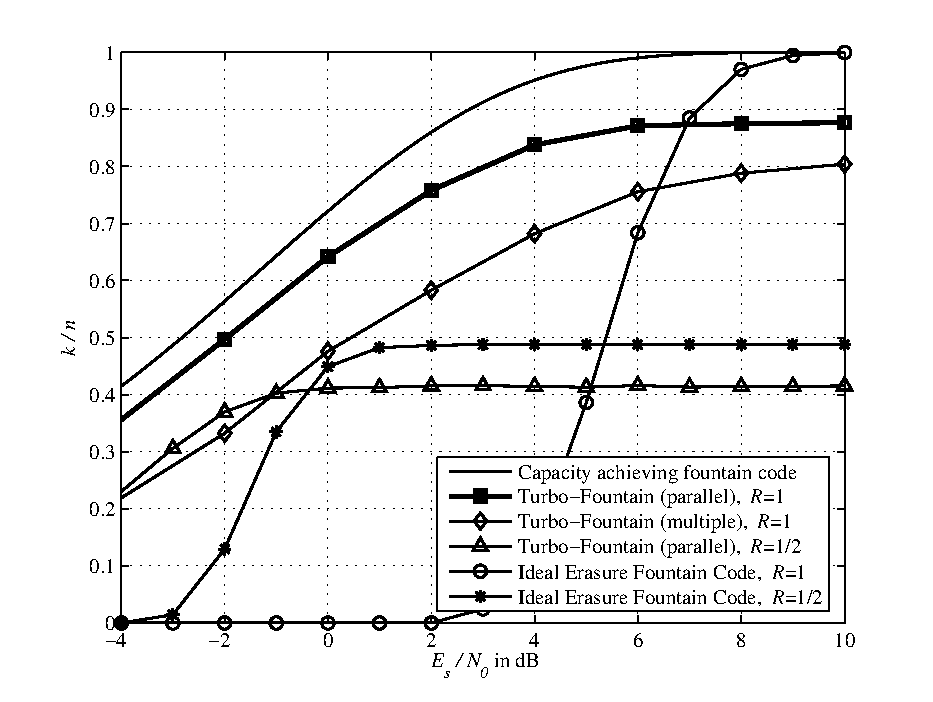
\includegraphics[width=\columnwidth]{plot_tf}
	% 	% Create a subtitle for the figure.
	% 	\caption{Simulation results on the AWGN channel. Average throughput $k/n$ vs $E_s/N_0$.}
	% 	% Define the label of the figure. It's good to use 'fig:title', so you know that the label belongs to a figure.
	% 	\label{fig:tf_plot}
	% 	\end{center}
	% \end{figure}


\section{Conclusion}

	% This section summarizes the paper. In our experiments, you can also write your gains and inspirations in here.
    Through this experiment, I learned how to solve problems using linear regression and linear classification, and learned how to use gradient descent to optimize the model. I learned that learning rate is an important hyperparameter, and if the learning rate is too large or too small, we can not get a good model.


% Your document ends here!
\end{document}